\appendix
\chapter{Allgemeines}

\newpage

\section{Zeitplan}

\begin{figure} [H]
	\begin{center}
		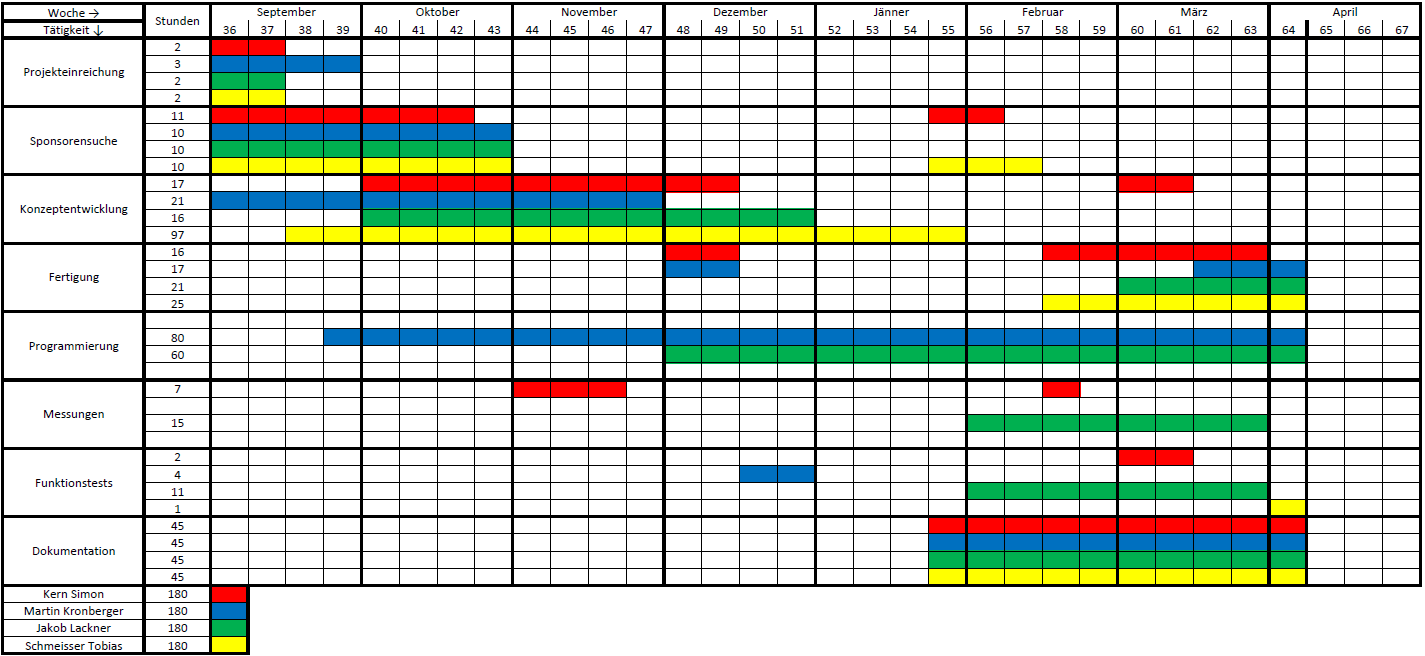
\includegraphics[angle=90, scale=0.6] {figures/allgemein/zeitplan.png}
		\caption{Zeitplan und Arbeitszeiten}
		\label{fig:Zeitplan}
	\end{center}
\end{figure}

\newpage

\section{Kosten}


\begin{figure} [H]
	\begin{center}
		\includegraphics[angle=-90, scale=0.6] {figures/allgemein/stückliste.png}
		\caption{Kostenaufstellung und Stückliste}
		\label{fig:Stückliste}
	\end{center}
\end{figure}

\newpage

\chapter{Programmcode}

\section{Antriebsstrang}
\definecolor{mGreen}{rgb}{0,0.6,0}
\definecolor{mGray}{rgb}{0.5,0.5,0.5}
\definecolor{mPurple}{rgb}{0.58,0,0.82}
\definecolor{backgroundColour}{rgb}{0.95,0.95,0.92}

\lstdefinestyle{CStyle}{
	backgroundcolor=\color{backgroundColour},   
	commentstyle=\color{mGreen},
	keywordstyle=\color{magenta},
	numberstyle=\tiny\color{mGray},
	stringstyle=\color{mPurple},
	basicstyle=\footnotesize,
	breakatwhitespace=false,         
	breaklines=true,                 
	captionpos=b,                    
	keepspaces=true,                 
	numbers=left,                    
	numbersep=5pt,                  
	showspaces=false,                
	showstringspaces=false,
	showtabs=false,                  
	tabsize=2,
	language=C
}



%\begin{document}
%	\begin{lstlisting}[style=CStyle]
%		#include <stdio.h>
%		int main(void)
%		{
%			printf("Hello World!"); 
%		}
%	\end{lstlisting}
%\end{document} 

\section{HICS}

\subsection{Benutzeroberfläche}




\chapter{CAD-Zeichnungen}

\newpage

\section{Mechanik}

\begin{figure} [H]
	\begin{center}
		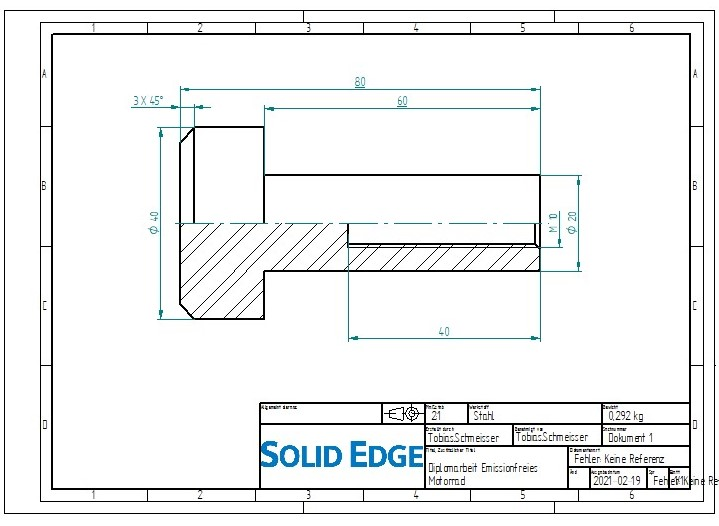
\includegraphics[angle=90, scale=0.9] {figures/mechanik/Welle_Rechts_Zeichnung.jpg}
		\caption{Wellenersatz}
		\label{fig:Wellenersatz1}
	\end{center}
\end{figure}

\newpage

\begin{figure} [H]
	\begin{center}
		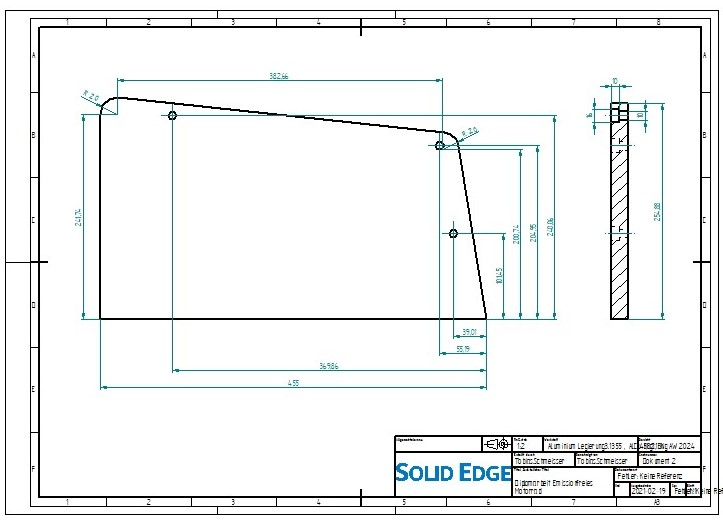
\includegraphics[angle=90]{figures/mechanik/Seitenplatte_Fertigung_Rechts.jpg}
		\caption{Seitenplatte Rechts}
		\label{fig:SeitenplatteRechts}
	\end{center}
\end{figure}

\begin{figure} [H]
	\begin{center}
		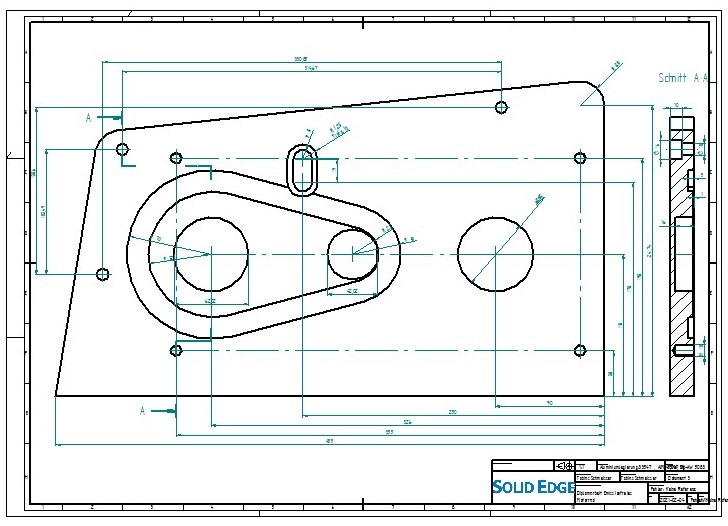
\includegraphics[angle=90]{figures/mechanik/Seitenplatte_Fertigung_Links.jpg}
		\caption{Seitenplatte Links}
		\label{fig:Seitenplatte Links}
	\end{center}
\end{figure}

\begin{figure} [H]
	\begin{center}
		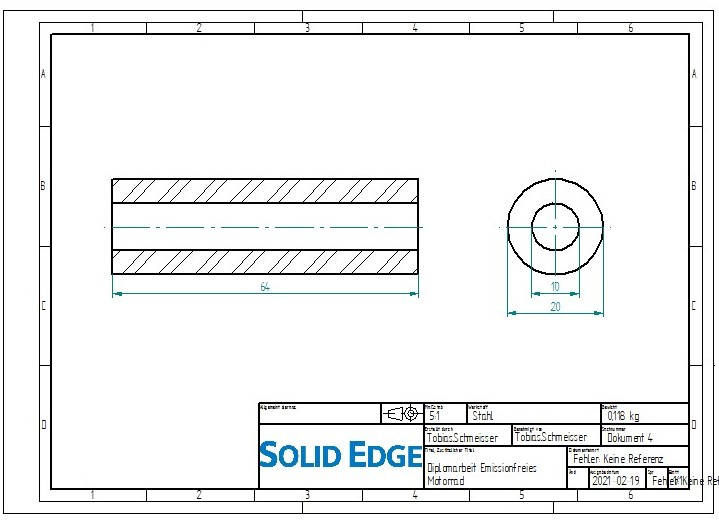
\includegraphics[angle=90]{figures/mechanik/Seitenplatte_Abstandhalter_Zeichnung.jpg}
		\caption{Abstandhalter}
		\label{fig:Abstandhalter}
	\end{center}
\end{figure}

\begin{figure} [H]
	\begin{center}
		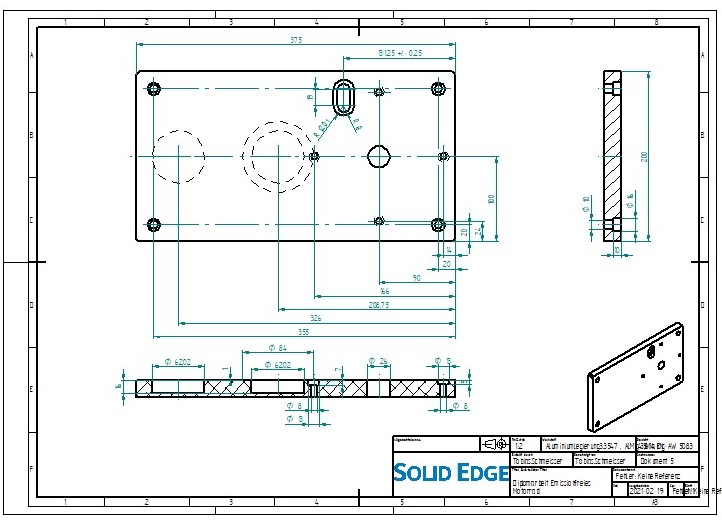
\includegraphics[angle=90]{figures/mechanik/Aufbau_Seitenplatte_Links_Zeichn.jpg}
		\caption{Aufbau/Zusatzplatte}
		\label{fig:Aufbau/Zusatzplatte}
	\end{center}
\end{figure}

\begin{figure} [H]
	\begin{center}
		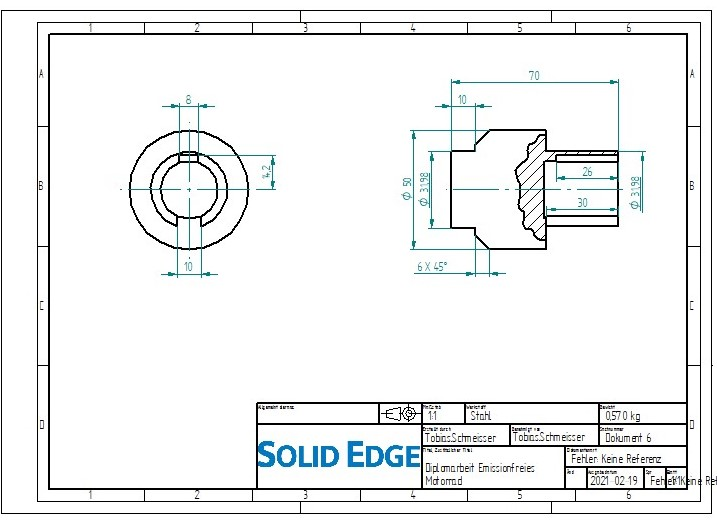
\includegraphics[angle=90]{figures/mechanik/Antriebsachse_Zeichnung.jpg}
		\caption{Achse 1/Antriebsachsen}
		\label{fig:Achse 1/Antriebsachsen}
	\end{center}
\end{figure}

\begin{figure} [H]
	\begin{center}
		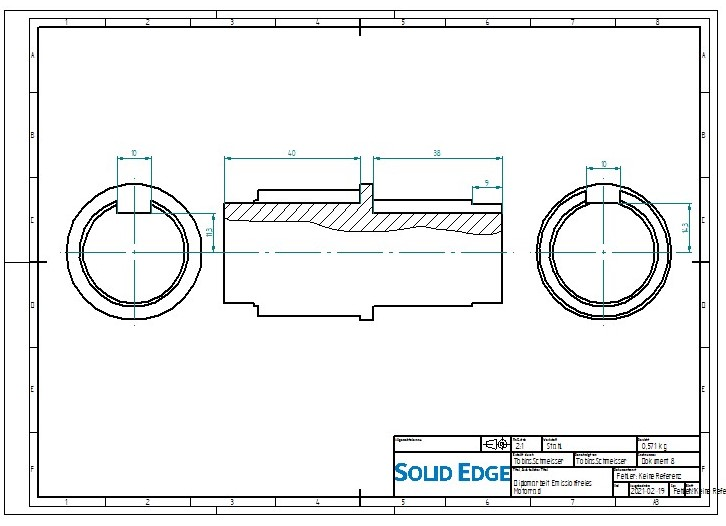
\includegraphics[angle=90]{figures/mechanik/Achse_mit_nuten_Zeichnung.jpg}
		\caption{Achse 3}
		\label{fig:Achse3}
	\end{center}
\end{figure}

\begin{figure} [H]
	\begin{center}
		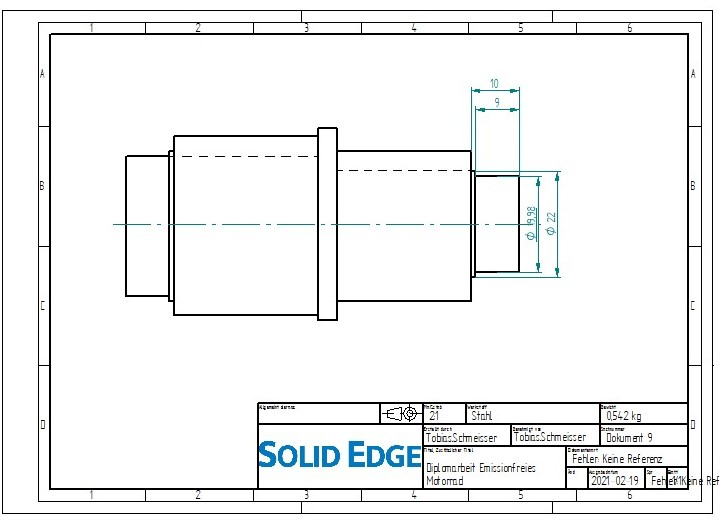
\includegraphics[angle=90]{figures/mechanik/Achse_mit_nuten_20mm_Zeichnung.jpg}
		\caption{Achse 2}
		\label{fig:Achse2}
	\end{center}
\end{figure}

\begin{figure} [H]
	\begin{center}
		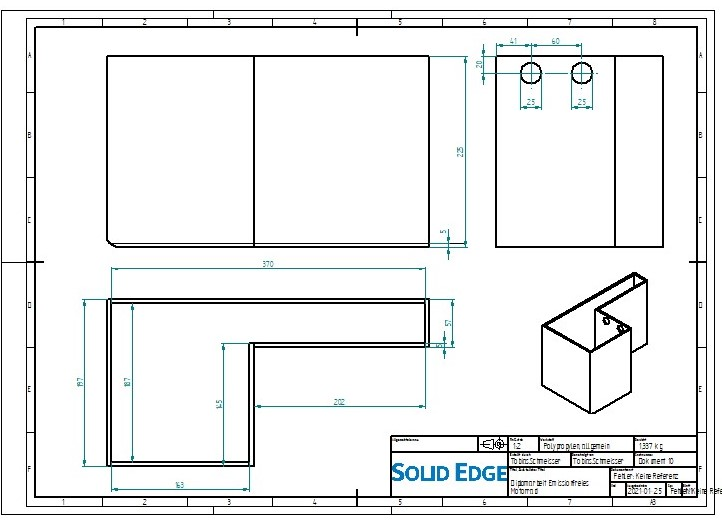
\includegraphics[angle=90]{figures/mechanik/Box_Zeichnung.jpg}
		\caption{Akkubox Motorblock}
		\label{fig:Akkubox Motorblock}
	\end{center}
\end{figure}

\begin{figure} [H]
	\begin{center}
		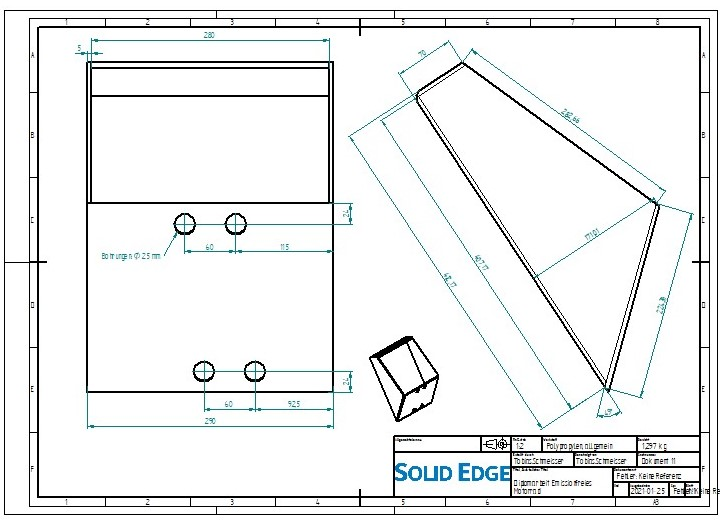
\includegraphics[angle=90]{figures/mechanik/Box_2_Zeichnung.jpg}
		\caption{Akkubox Vorderseite}
		\label{fig:Akkubox Vorderseite}
	\end{center}
\end{figure}

\begin{figure} [H]
	\begin{center}
		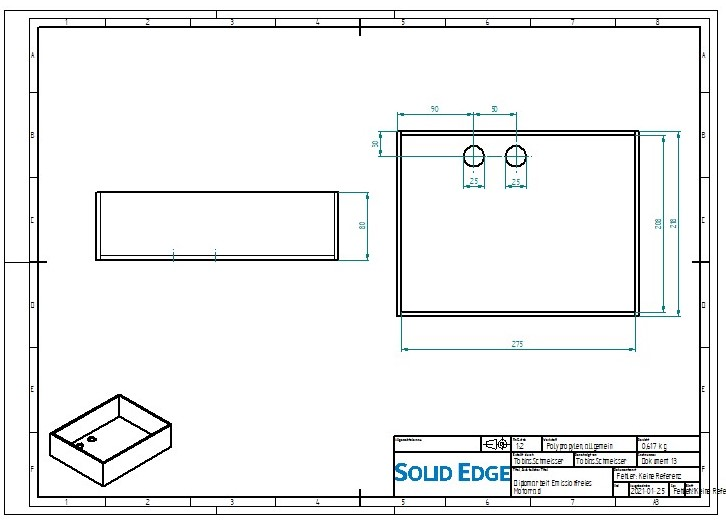
\includegraphics[angle=90]{figures/mechanik/Box_3_Zeichnung.jpg}
		\caption{Akkubox Mitte}
		\label{fig:Akkubox Mitte}
	\end{center}
\end{figure}

\section{Antriebsstrang}
\begin{figure} [H]
	\begin{center}
		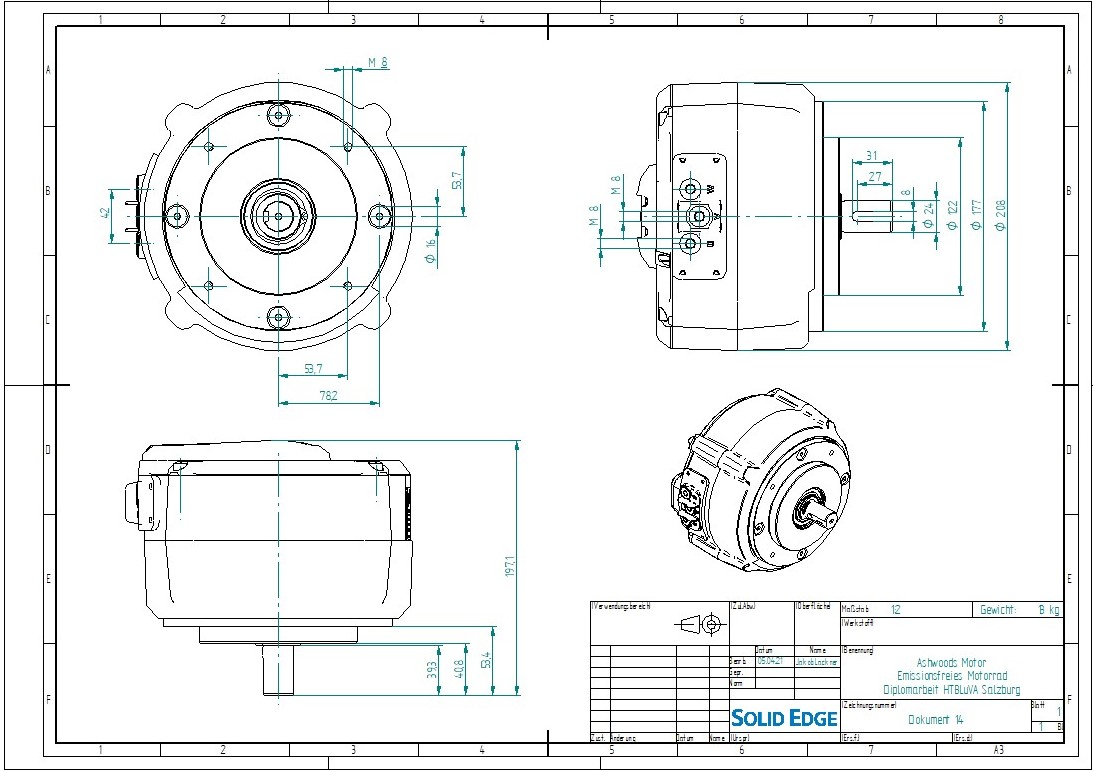
\includegraphics[angle=90, width=\textwidth]{figures/antrieb/Ashwoods_CAD.jpg}
		\caption{Ashwoods Motor}
		\label{Ashwoods_CAD}
	\end{center}
\end{figure}

\begin{figure} [H]
	\begin{center}
		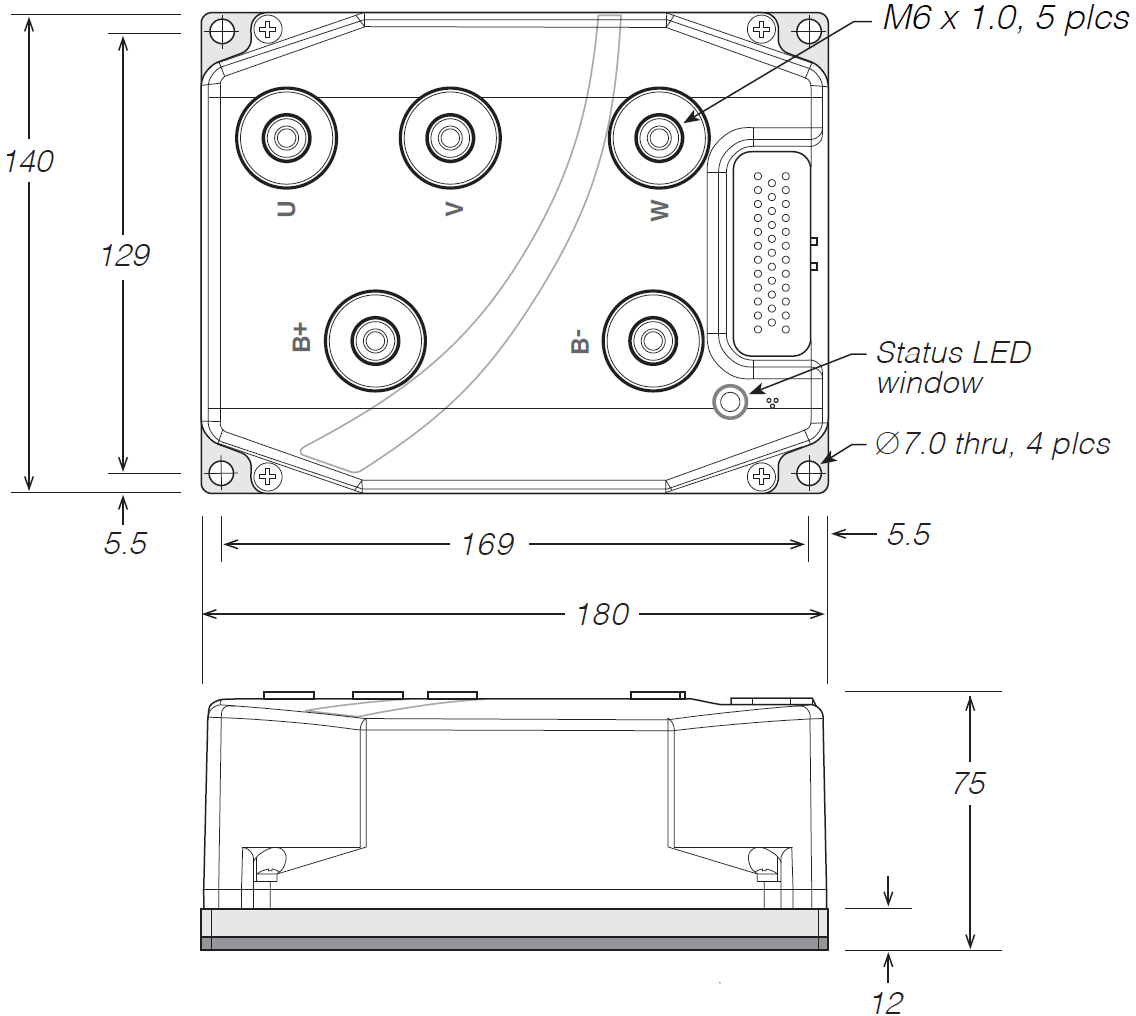
\includegraphics[width=1.05\textwidth]{figures/antrieb/Curtis_CAD.png}
		\caption{Curtis Controller}
		\label{Curtis_CAD}
	\end{center}
\end{figure}

\section{HCIS} \label{app:hcis}
\begin{figure} [H]
	\begin{center}
		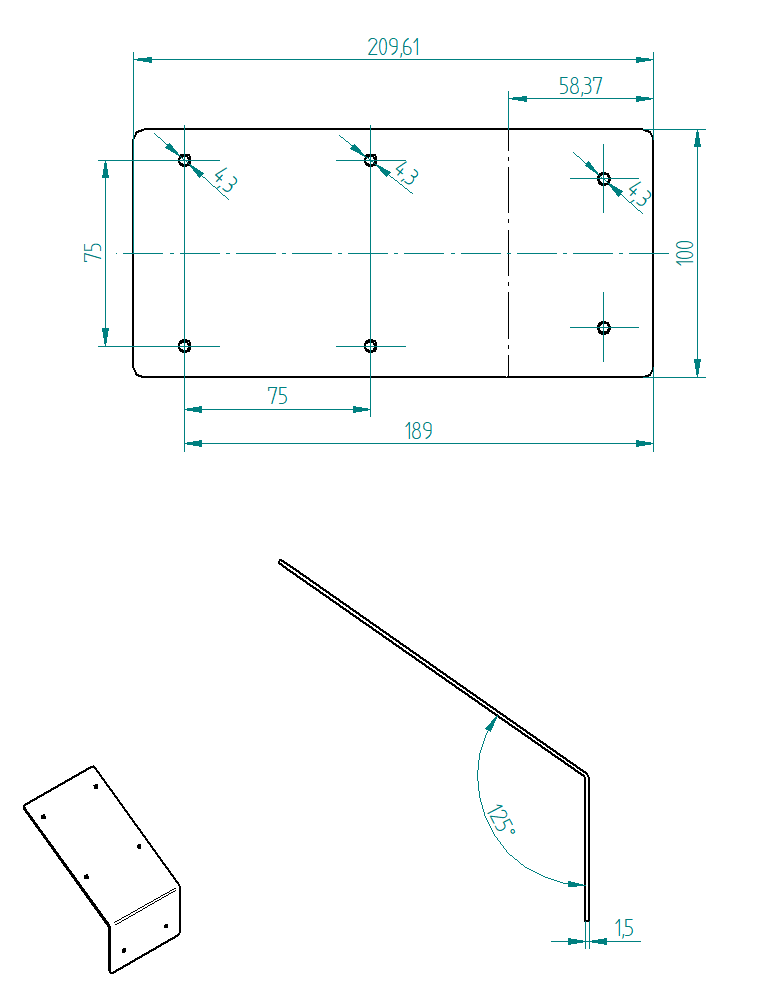
\includegraphics[scale=0.8]{figures/hcis/befestigung_display_cad.png}
		\caption{Akkubox Mitte}
		\label{fig:panel_cad}
	\end{center}
\end{figure}

\chapter{Simulationen}

\section{Mechanik}

\fancyfoot[C]{Schmeisser}

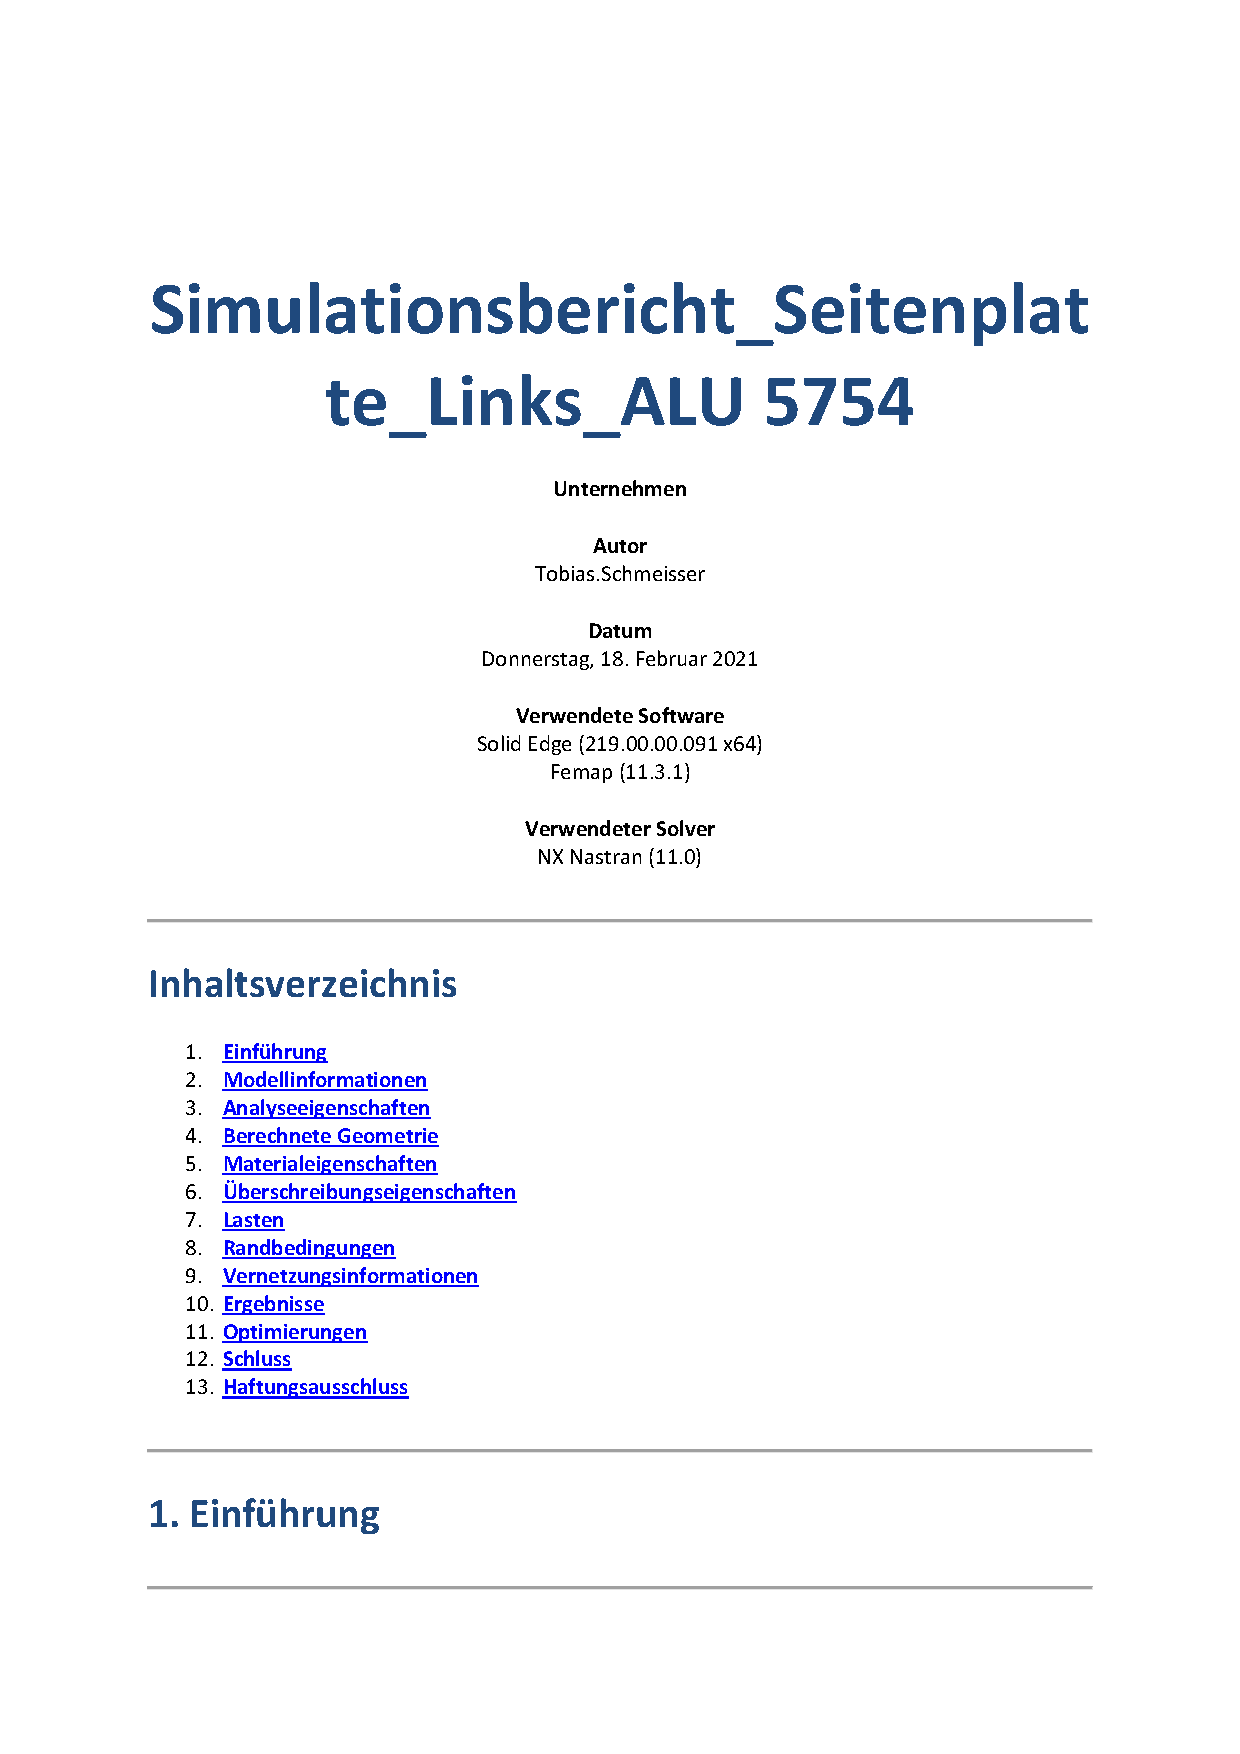
\includepdf[pages=-, pagecommand={\thispagestyle{fancy}}, scale=0.95] {figures/mechanik/Simulationen/Seitenplatte_Links_Statische Berechnung 1_3.pdf}

\includepdf[pages=-, pagecommand={\thispagestyle{fancy}}, scale=0.95] {figures/mechanik/Simulationen/Seitenplatte_Rechts_Statische Berechnung 1_3.pdf}

\newpage

\chapter{Schaltpläne}

\section{Antriebsstrang}
\begin{figure}[H]
	\begin{center}
		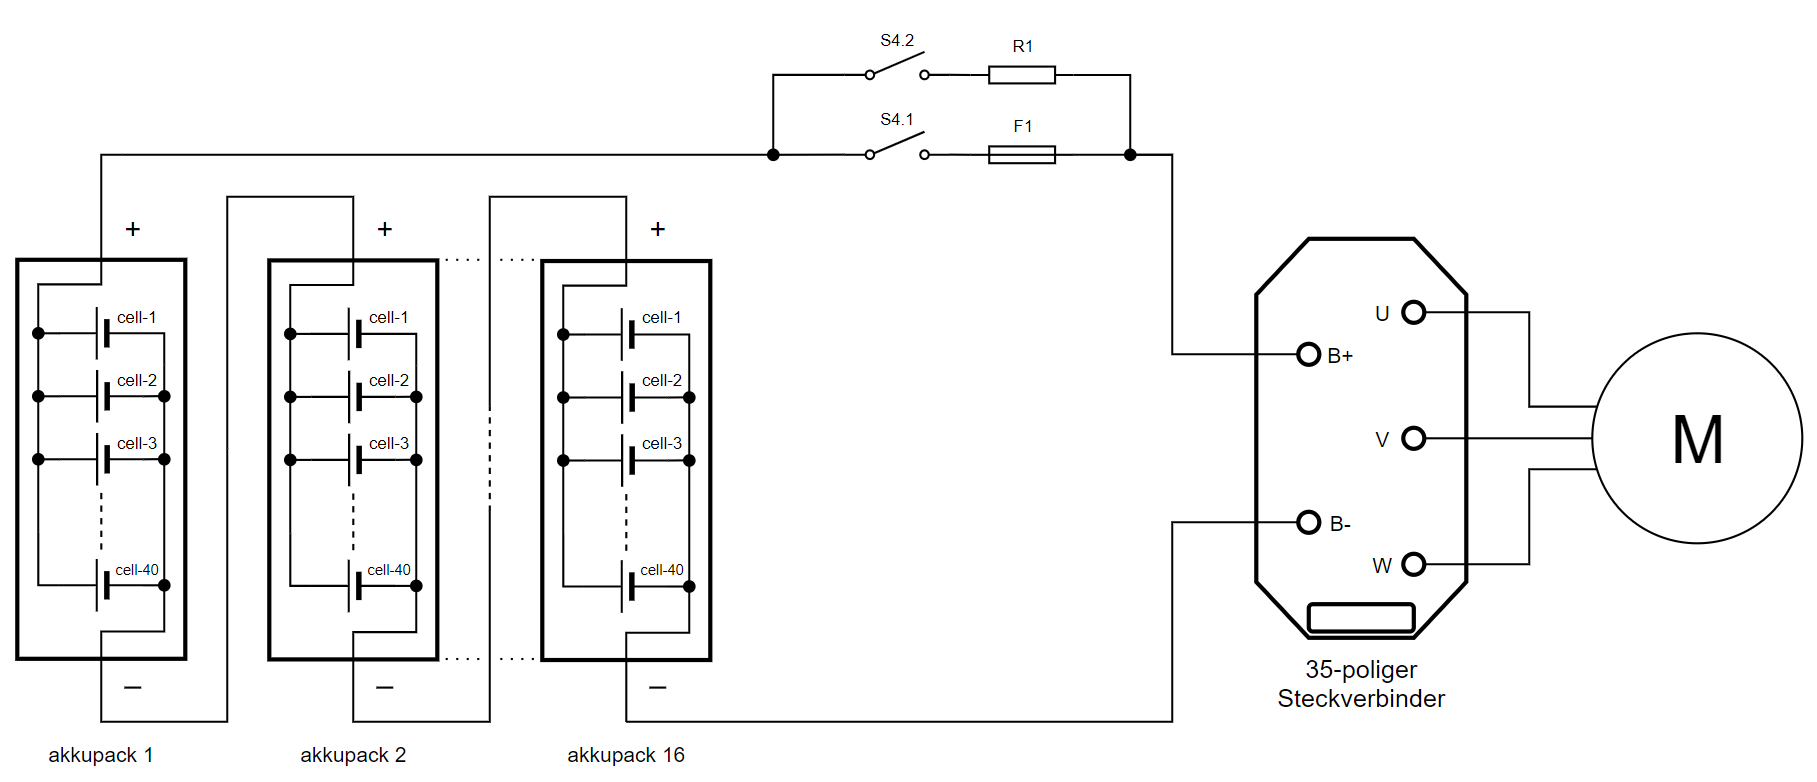
\includegraphics[scale=0.35]{figures/Antrieb/Antrieb_Laststromkreis.png}
		\caption{Grundaufbau des Laststromkreises}
		\label{Grundaufbau_Laststromkreis}
	\end{center}
\end{figure}

\begin{figure}[H]
	\begin{center}
		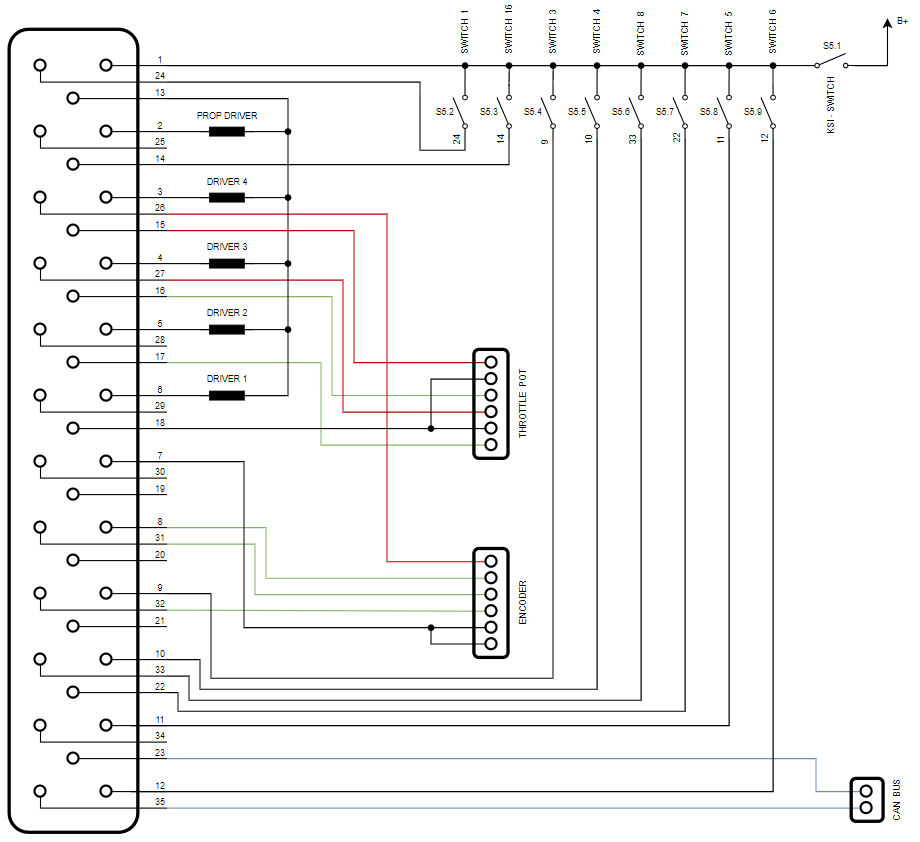
\includegraphics[scale=0.67]{figures/Antrieb/Antrieb_Steuerstromkreis.png}
		\caption{Grundaufbau des Steuerstromkreises}
		\label{Grundaufbau_Steuerstromkreis}
	\end{center}
\end{figure}

\newpage

\section{HCIS}

\newpage

\chapter{Datenblätter}

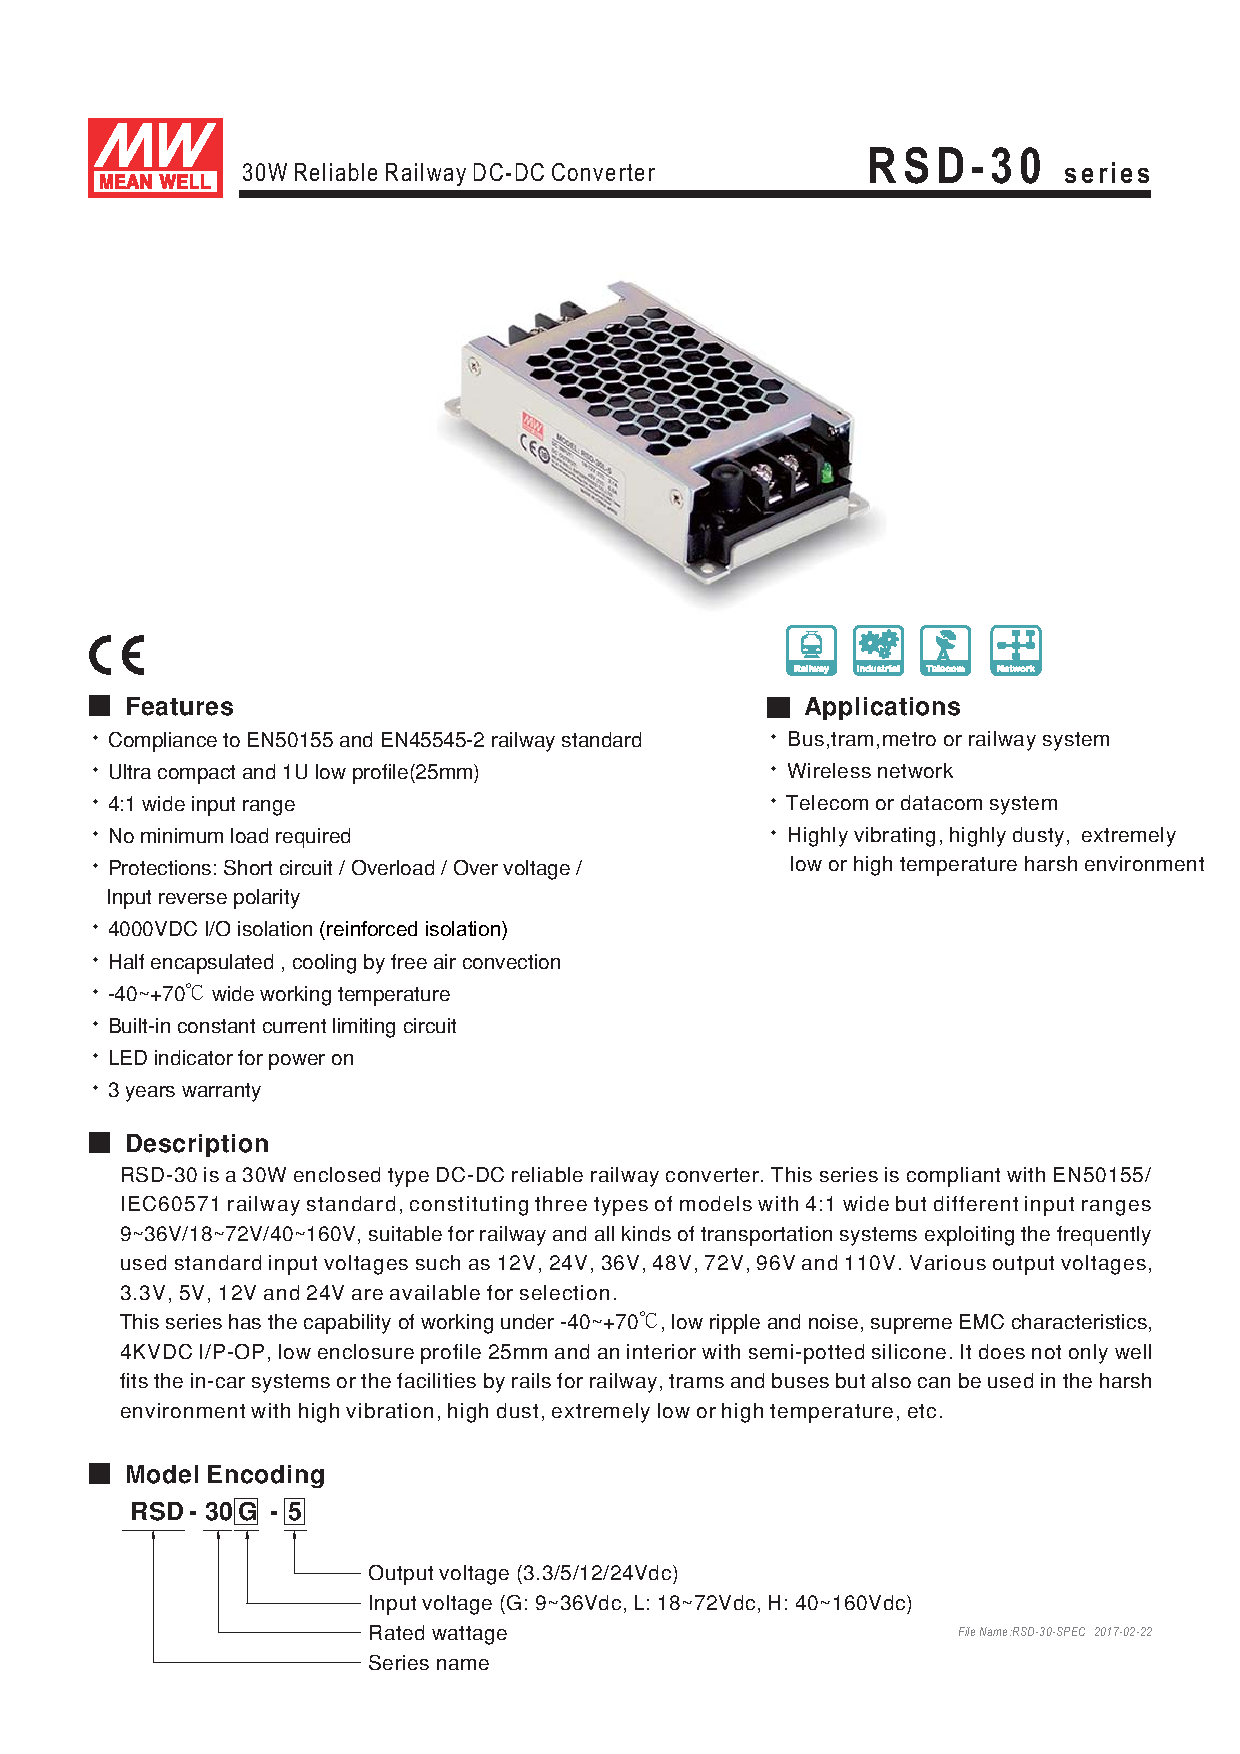
\includepdf[pages=1, pagecommand={\thispagestyle{fancy}}, pagecommand={\section{HCIS} \subsection{Mean Well RSD-30H-5} \label{app:mw5}}, scale=0.8] {pdf/meanwell5.pdf}
\includepdf[pages=2-, pagecommand={\thispagestyle{fancy}}, scale=0.95] {pdf/meanwell5.pdf}


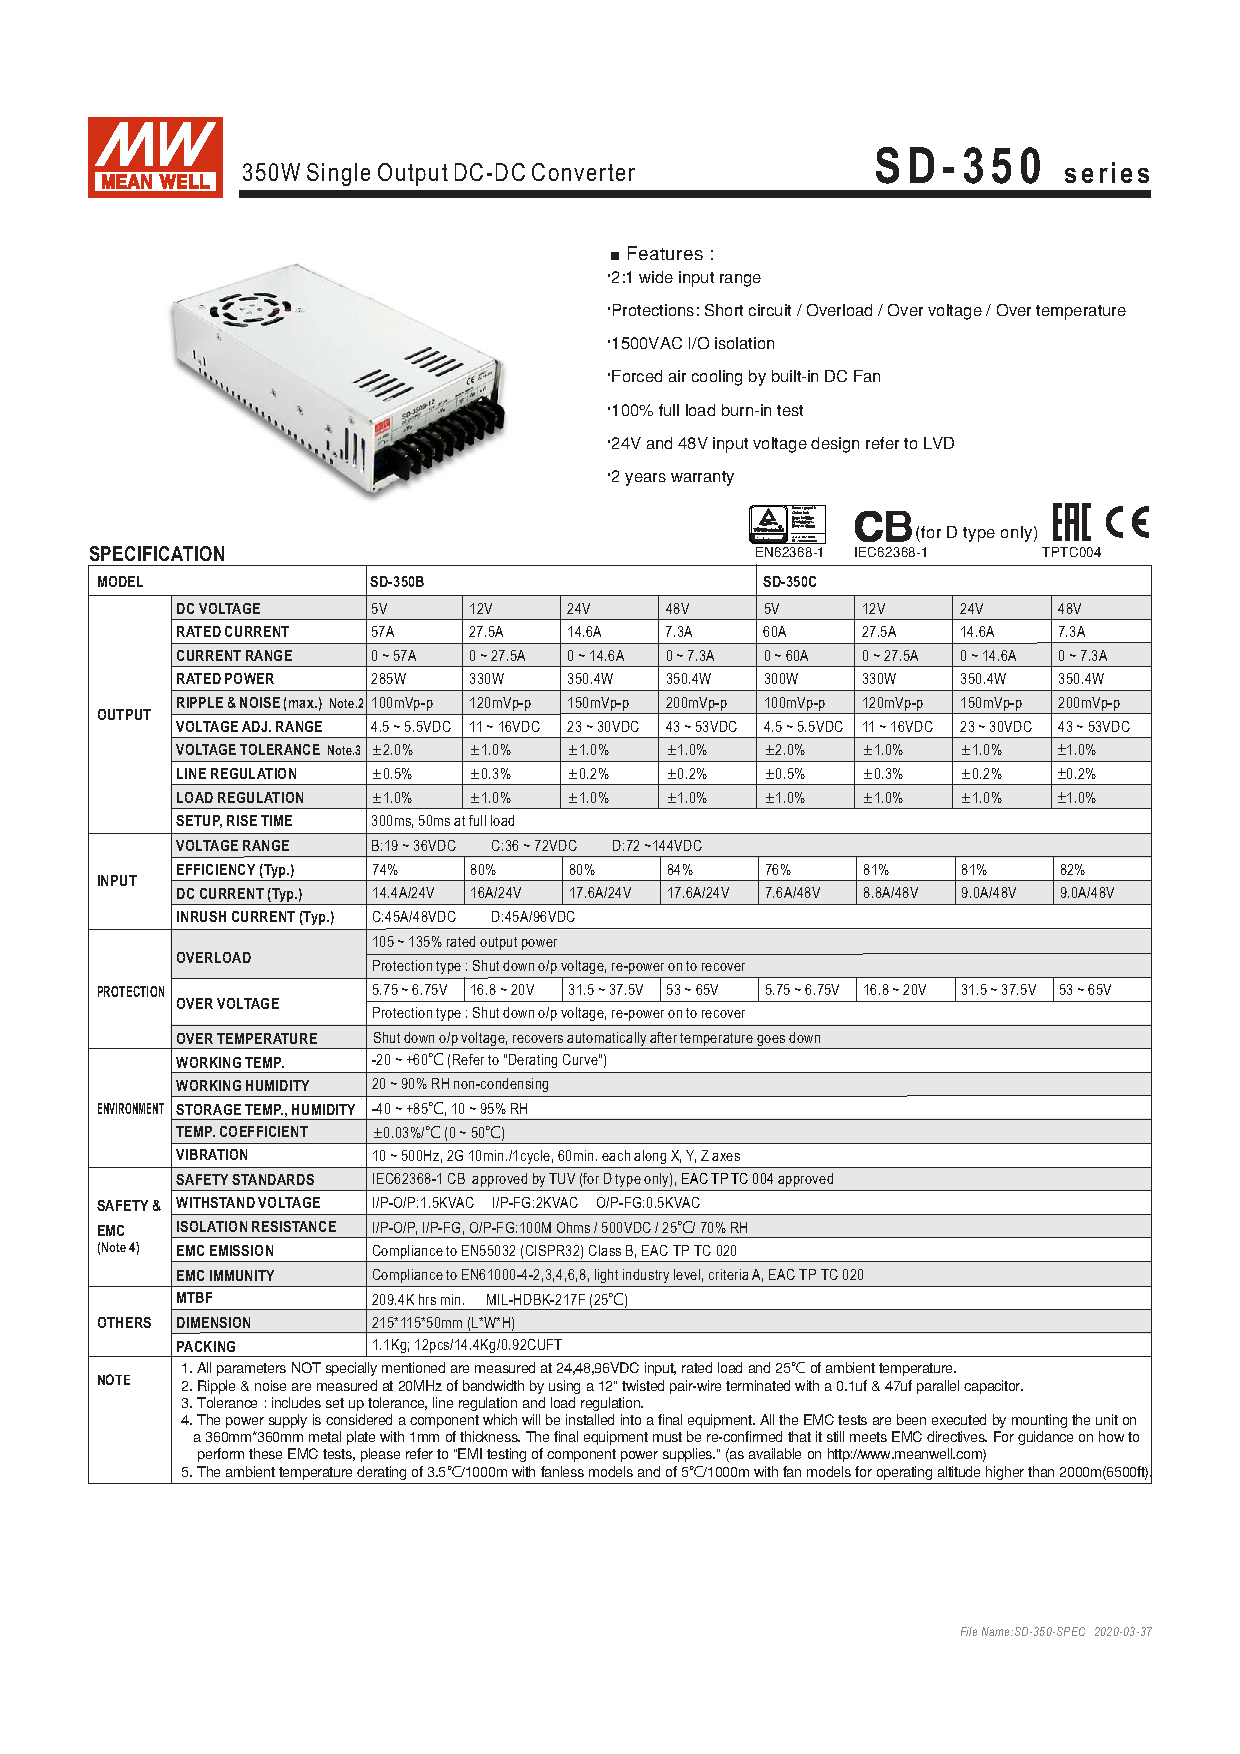
\includepdf[pages=1, pagecommand={\thispagestyle{fancy}}, pagecommand={\subsection{Mean Well SD-350C-12} \label{app:mw12}}, scale=0.8] {pdf/meanwell12.pdf}
\includepdf[pages=2-, pagecommand={\thispagestyle{fancy}}, scale=0.95] {pdf/meanwell12.pdf}


\includepdf[pages=1, pagecommand={\thispagestyle{fancy}}, pagecommand={\subsection{Raspberry Pi 4 Moddel B} \label{app:rasp}}, scale=0.8] {pdf/raspberry.pdf}

\includepdf[pages=2-, pagecommand={\thispagestyle{fancy}}, scale=0.95] {pdf/raspberry.pdf}

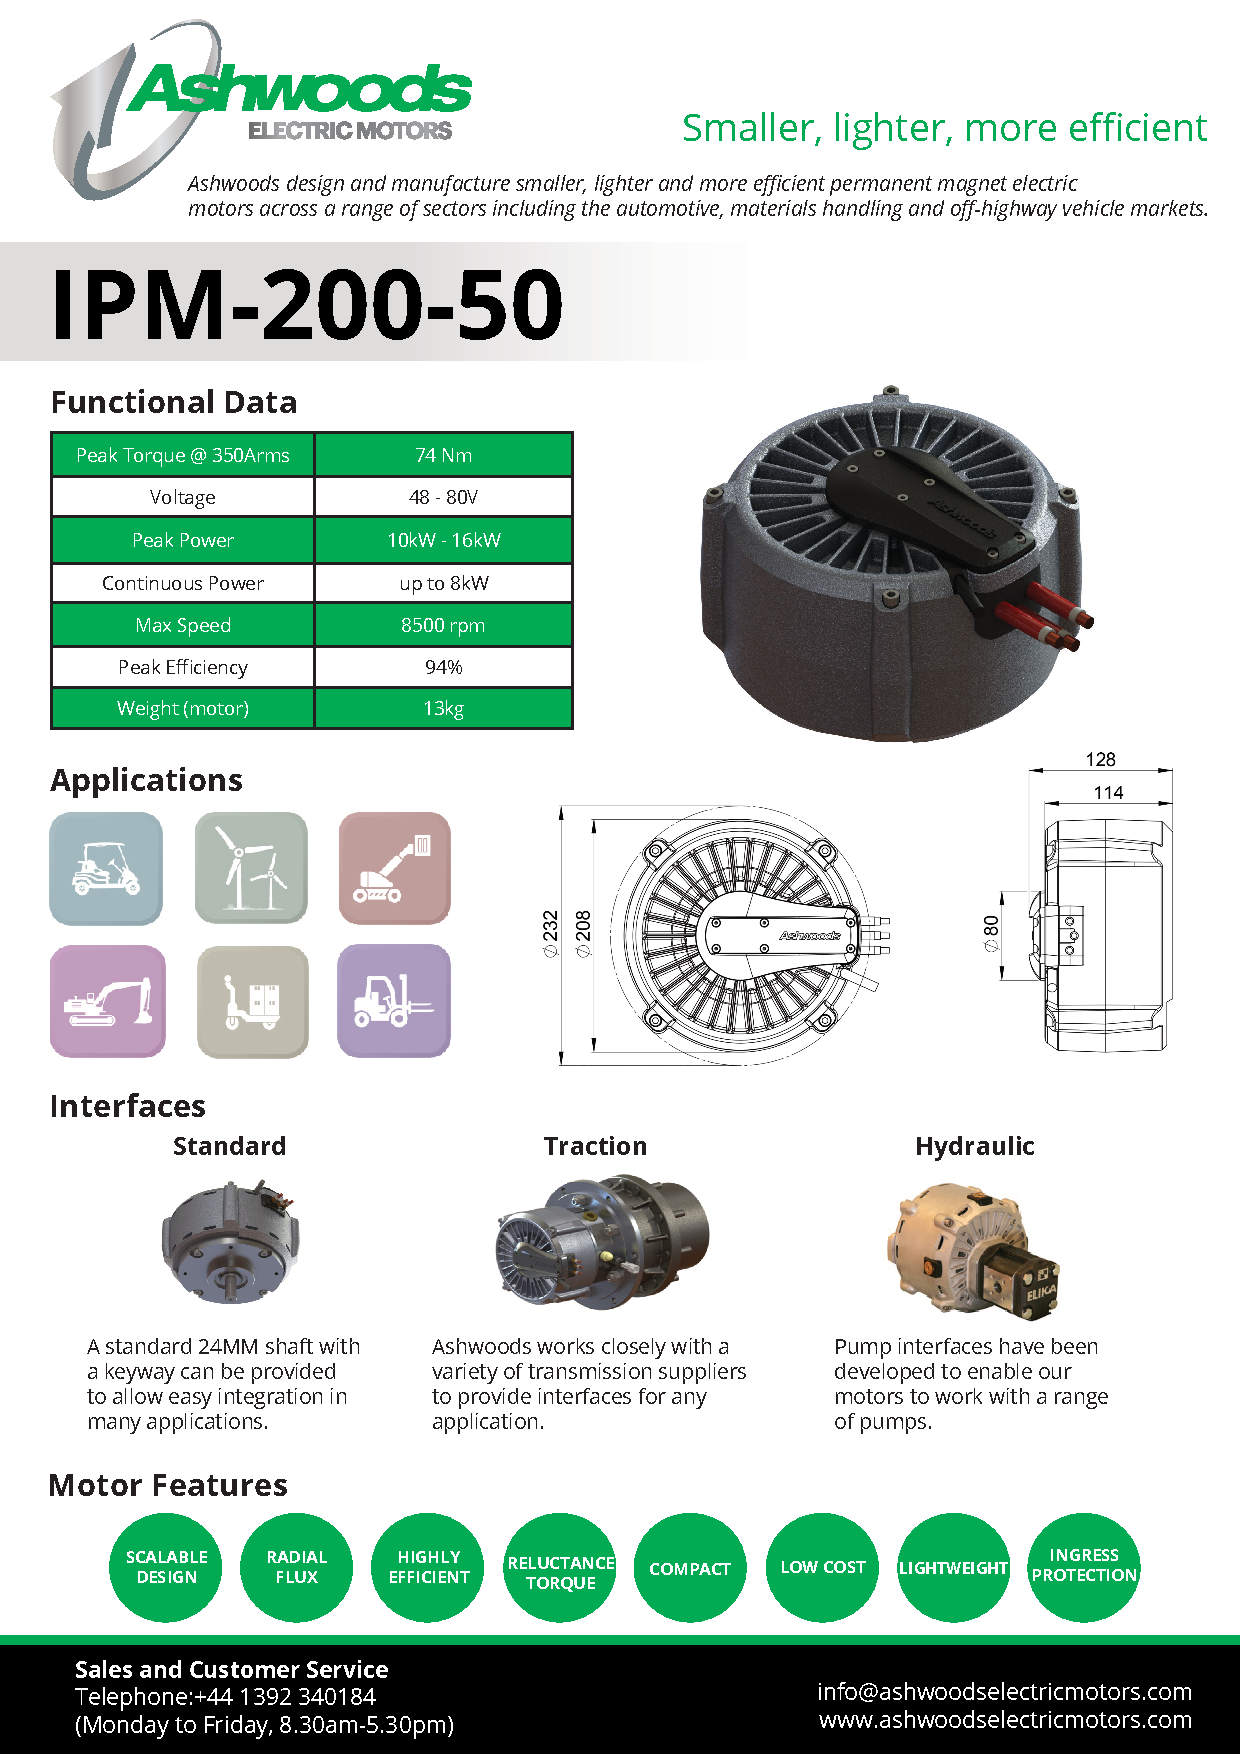
\includepdf[pages=1, pagecommand={\thispagestyle{fancy}}, pagecommand={\section{Antrieb}\subsection{Ashwoods Elektro-Motor IPM-200-50} 
\label{Ashwoods_Motor}}, scale=0.75] {pdf/Ashwoods_IPM-200-50.pdf}
\includepdf[pages=2-, pagecommand={\thispagestyle{fancy}}, scale=0.8] {pdf/Ashwoods_IPM-200-50.pdf}

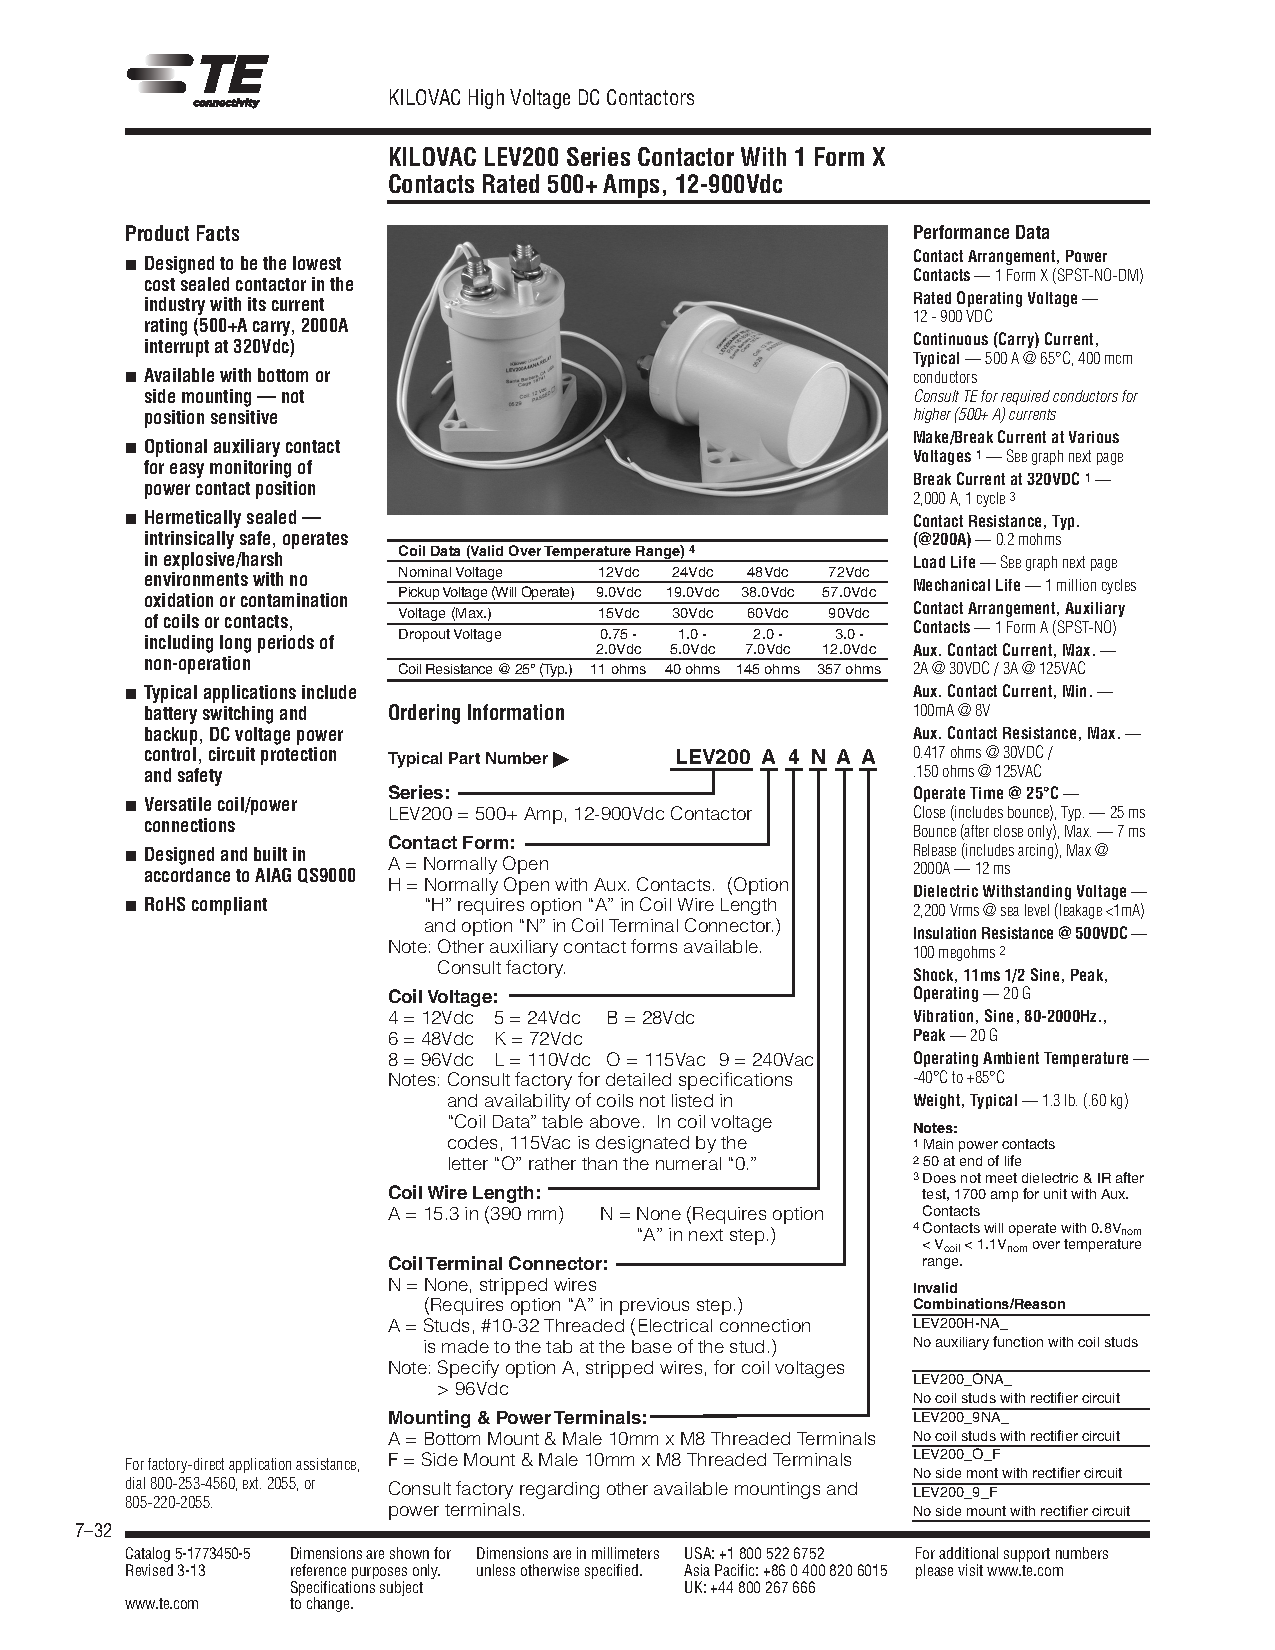
\includepdf[pages=1, pagecommand={\thispagestyle{fancy}}, pagecommand={\subsection{Hochleistungs-Relais: KILOVAC LEV200 A4ANA} 
\label{KILOVAC_LEV200_A4ANA}}, scale=0.85] {pdf/KILOVAC_LEV200_A4ANA.pdf}
\includepdf[pages=2, pagecommand={\thispagestyle{fancy}}, scale=0.9] {pdf/KILOVAC_LEV200_A4ANA.pdf}

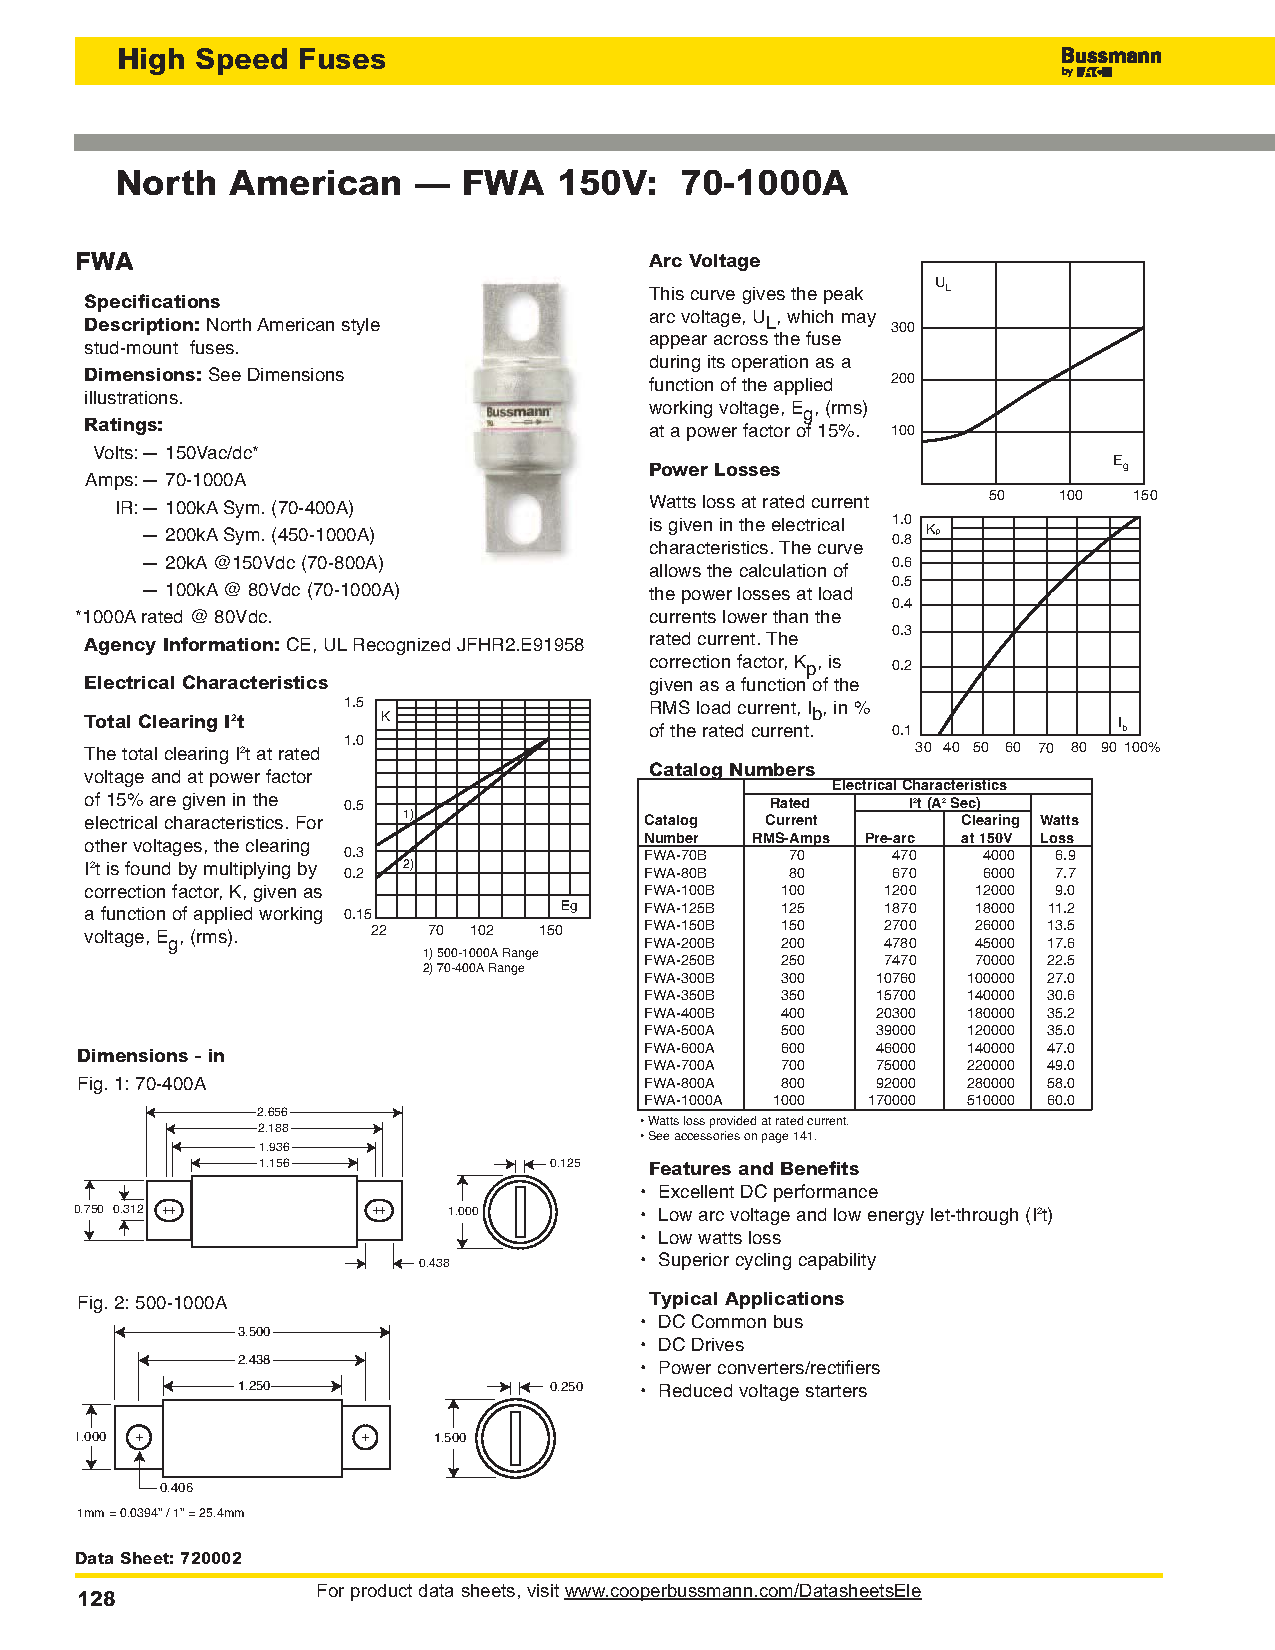
\includepdf[pages=1, pagecommand={\thispagestyle{fancy}}, pagecommand={\subsection{Hochgeschwindigkeits-Schmelzsicherung: FWA-400B} \label{FWA-400B}}, scale=0.82] {pdf/FWA-400B.pdf}
\includepdf[pages=2-, pagecommand={\thispagestyle{fancy}}, scale=0.85] {pdf/FWA-400B.pdf}

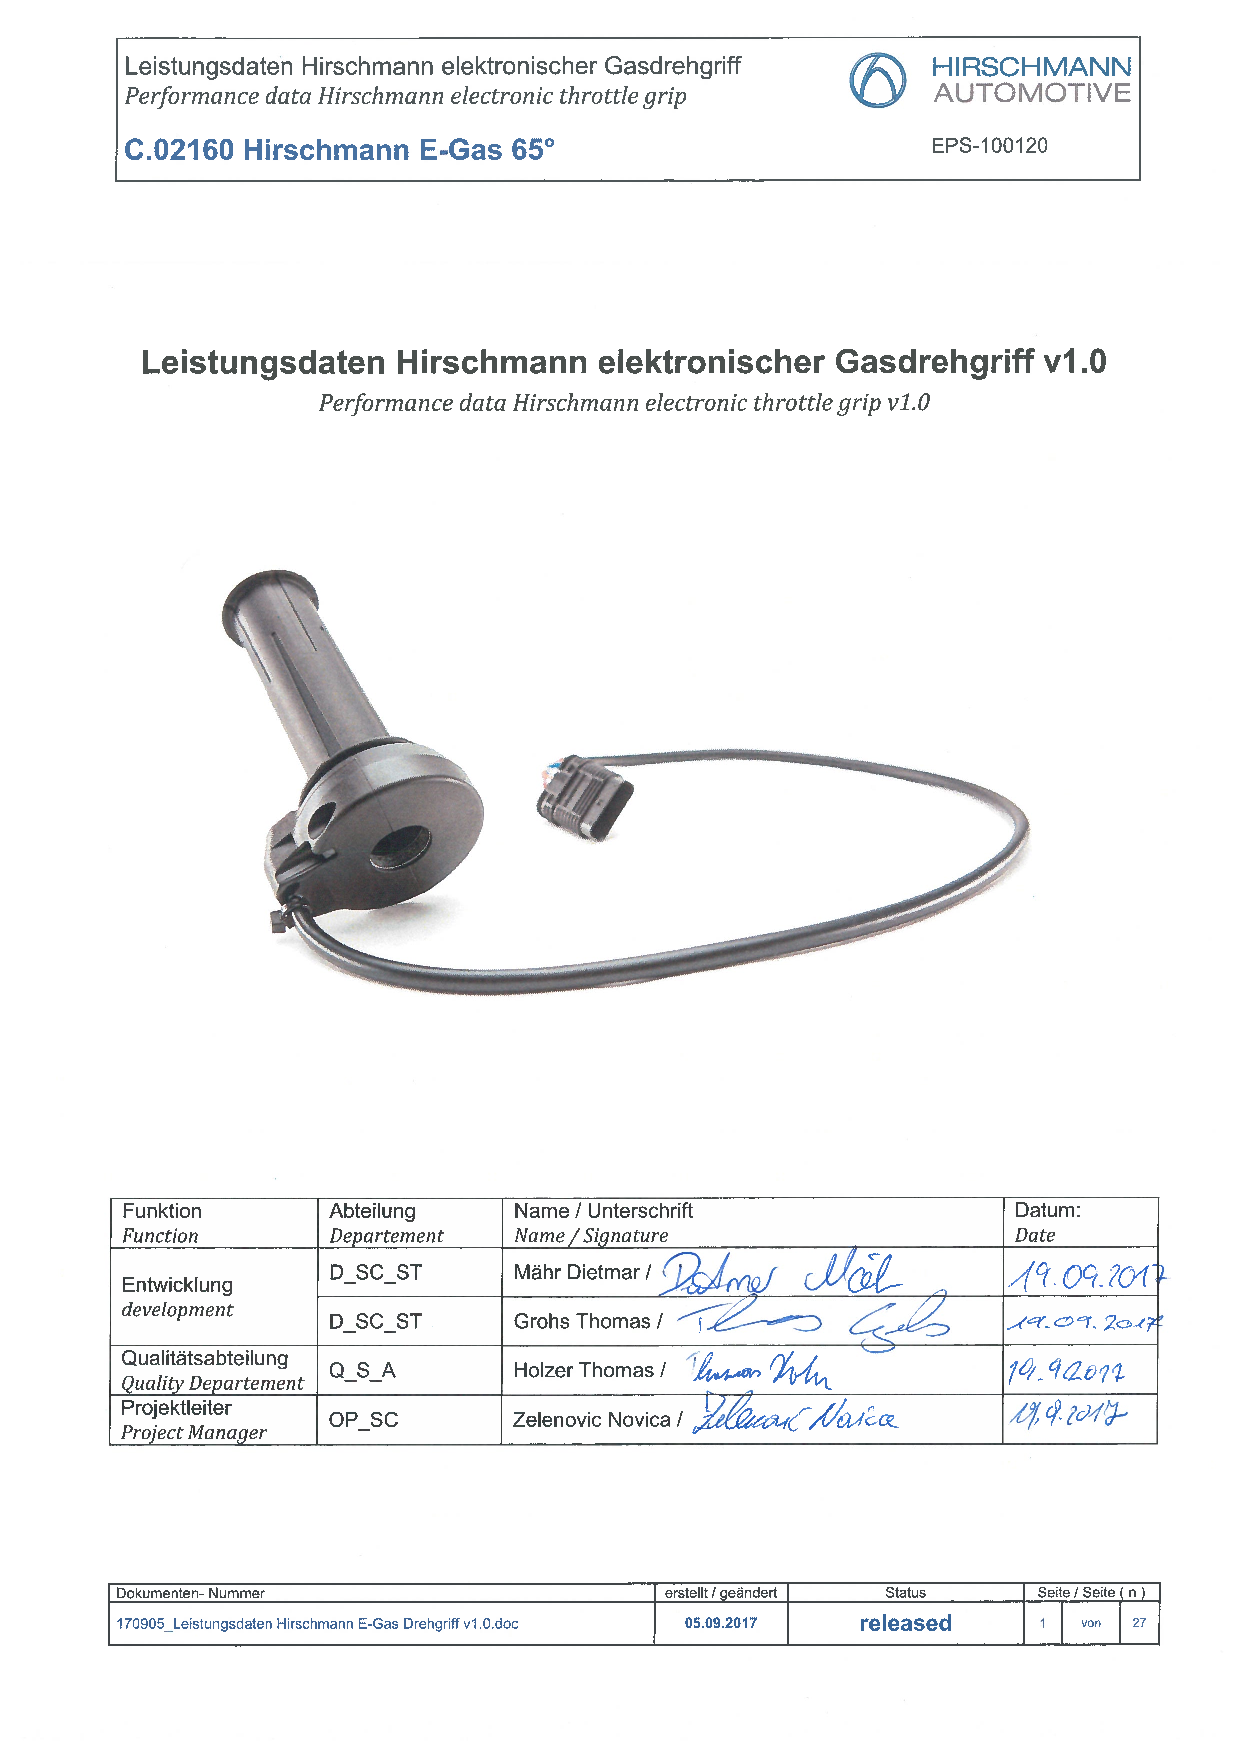
\includepdf[pages=1, pagecommand={\thispagestyle{fancy}}, pagecommand={\subsection{Leistungsdaten Hirschmann elektronischer Gasdrehgriff v1.0} \label{Hirschmann_E-Gas_Drehgriff}}, scale=0.8] {pdf/Leistungsdaten_Hirschmann_E-Gas_Drehgriff.pdf}
\includepdf[pages=2-, pagecommand={\thispagestyle{fancy}}, scale=0.85] {pdf/Leistungsdaten_Hirschmann_E-Gas_Drehgriff.pdf}

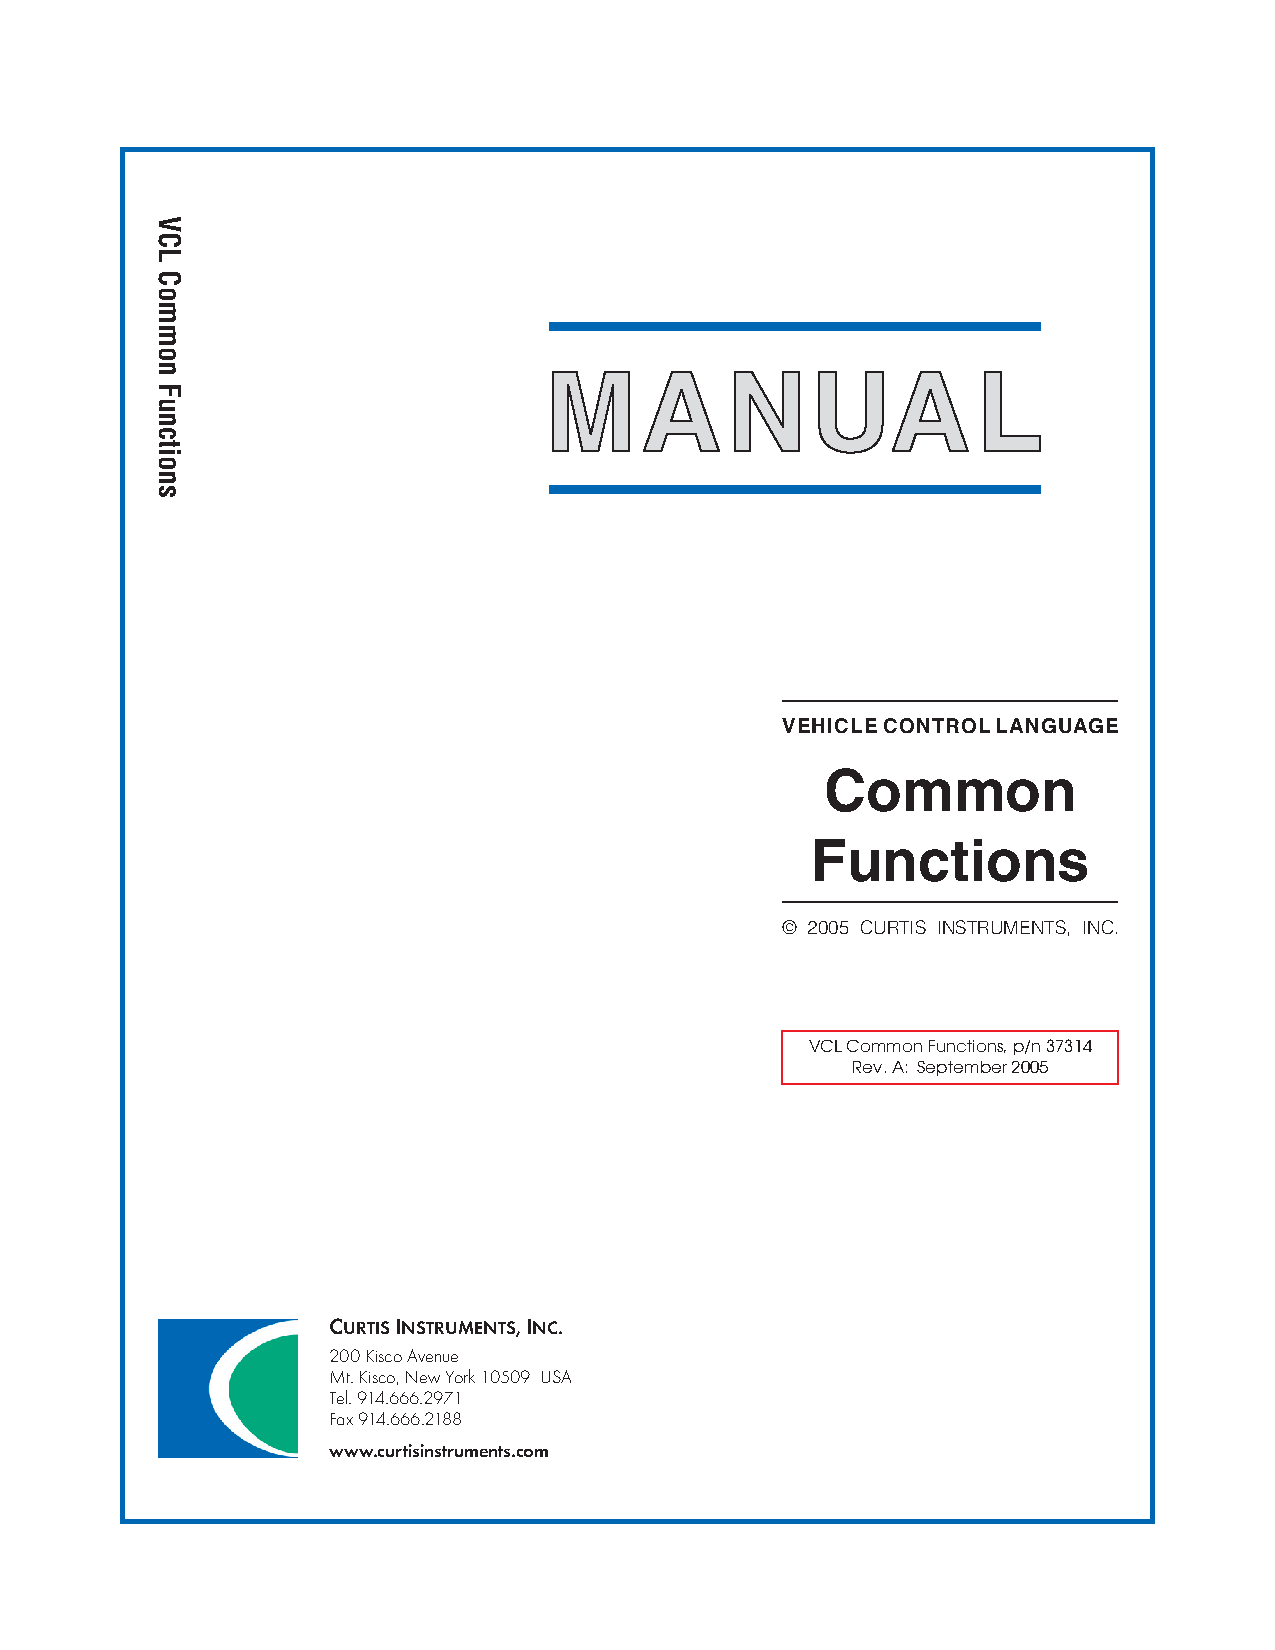
\includepdf[pages=1, pagecommand={\thispagestyle{fancy}}, pagecommand={\subsection{VCL Common Functions} \label{VCL_Common_Functions}}, scale=0.8] {pdf/VCL_Common_Functions.pdf}
\includepdf[pages=3-7, pagecommand={\thispagestyle{fancy}}, scale=0.85] {pdf/VCL_Common_Functions.pdf}
\includepdf[pages=31-33, pagecommand={\thispagestyle{fancy}}, scale=0.85] {pdf/VCL_Common_Functions.pdf}
\includepdf[pages=48-52, pagecommand={\thispagestyle{fancy}}, scale=0.85] {pdf/VCL_Common_Functions.pdf}
\includepdf[pages=70-89, pagecommand={\thispagestyle{fancy}}, scale=0.85] {pdf/VCL_Common_Functions.pdf}